\input{preamble_ask.tex}
\input{definitions_ask.tex}


\pagestyle{askhseis}
\everymath{\displaystyle}

\begin{document}

\begin{center}
\minibox{\large\bfseries \textcolor{Col1}{Επικαμπύλιο Ολοκλήρωμα Ιου είδους}}
\end{center}

\vspace{\baselineskip}


\begin{enumerate}
  \item Να υπολογιστούν τα παρακάτω επικαμπύλια ολοκληρώματα κατά μήκος των 
    δοσμένων καμπυλών:
    \begin{enumerate}[i)]
      %thomas ex.9 p. 906
      \item $ \int _{c} (x+y) \,{ds} $, όπου $ c \colon $ καμπύλη με 
        παραμ. εξισώσεις $ x=t $, $ y=1-t $, $ z=0 $ από $ A(0,1,0) $ έως $B(1,0,0)$. 
        \hfill Απ: $ \sqrt{2} $ 
      %thomas ex.10 p. 906
      \item $ \int _{c} (x-y+z-2) \,{ds} $, όπου $ c \colon $ το ευθύγραμμο τμήμα 
        από το σημείο $ A(0,1,1) $ έως $ B(1,0,1) $.
        \hfill Απ: $ -\sqrt{2} $ 
      %thomas ex.11 p. 906
      \item $ \int _{c} (xy+y+z) \,{ds} $, όπου $ c \colon $ καμπύλη 
        $ \mathbf{r}(t)=2t\, \mathbf{i} + t\, \mathbf{j} + (2-2t) \, \mathbf{k} $, 
        με $ 0 \leq t \leq 1 $.  
        \hfill Απ: $13/2$ 
      %thomas ex.12 p. 906
      \item $ \int _{c} \sqrt{x^{2}+y^{2}} \,{ds} $, όπου $ c \colon $ έλικα με 
        $ \mathbf{r}(t)=(4 \cos{t} )\, \mathbf{i} + (4 \sin{t})\, \mathbf{j} + 3t \, 
        \mathbf{k} $, με $ -2 \pi \leq t \leq 2 \pi $.  
        \hfill Απ: $80 \pi$ 
      %thomas ex.14 p. 906
      \item $ \int _{c} \frac{\sqrt{3}}{x^{2}+y^{2}+z^{2}}\,{ds} $, όπου $ c \colon $ 
        $ \mathbf{r}(t)= t\, \mathbf{i} + t\, \mathbf{j} + t\, 
        \mathbf{k} $, με $1 \leq t \leq \infty$.  
        \hfill Απ: $1$ 
      %thomas ex.27 p. 906
      \item $ \int _{c} x^{3}/y \,{ds} $, όπου $ c \colon y=x^{2}/2 $ με 
        $0 \leq x \leq 2$.  
        \hfill Απ: $ \frac{10 \sqrt{5} -2}{3} $ 
      %thomas ex.29 p. 906
      \item $ \int _{c} (x+y) \,{ds} $, όπου $ c \colon x^{2}+y^{2}=4 $ στο 1ο
        τεταρτημόριο.  \hfill Απ: $8$ 
        %spand
      \item $ \int _{c} (x+y) \,{ds} $, όπου $ c \colon $ η περίμετρος τριγώνου 
        με κορυφές $ A(1,0) $, $ B(0,1) $, $ O(0,0) $.
        \hfill Απ: $ \sqrt{2} +1 $ 

    \end{enumerate}

  \item Να υπολογιστούν τα παρακάτω επικαμπύλια ολοκληρώματα. 
    \begin{enumerate}[i)]
      \item $ \int _{c} (x+ \sqrt{y}) \,{ds} $, όπου $ c \colon $ η καμπύλης του 
        σχήματος.
        \hfill Απ: $ \frac{5}{6} \sqrt{5} + \frac{3}{2} $ 

        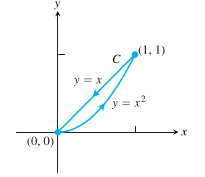
\includegraphics[scale=0.5]{int2.png}

    \end{enumerate}


\end{enumerate}



\end{document}
